\documentclass[t]{beamer}
\usepackage[utf8]{inputenc}  % to be able to type unicode text directly
%\usepackage[french]{babel}   % french typographical conventions
\usepackage{inconsolata}     % for a nicer (e.g. non-courier) tt family font
%\usepackage{amsthm,amsmath}  % fancier mathematics
\usepackage{array} % to fine-tune tabular spacing
\usepackage{bbm} % for blackboard 1

\usepackage{graphicx}        % to include images
%\usepackage{animate}         % to include animated images
\usepackage{soul}            % for colored strikethrough
%\usepackage{bbding}          % for Checkmark and XSolidBrush
\usepackage{hyperref,url}

\colorlet{darkgreen}{black!50!green}  % used for page numbers
\definecolor{term}{rgb}{.9,.9,.9}     % used for code insets

\setlength{\parindent}{0em}
\setlength{\parskip}{1em}


% coco's macros
\def\R{\mathbf{R}}
\def\F{\mathcal{F}}
\def\x{\mathbf{x}}
\def\y{\mathbf{y}}
\def\u{\mathbf{u}}
\def\Z{\mathbf{Z}}
\def\d{\mathrm{d}}
\DeclareMathOperator*{\argmin}{arg\,min}
\DeclareMathOperator*{\argmax}{arg\,max}
\newcommand{\reference}[1] {{\scriptsize \color{gray}  #1 }}
\newcommand{\referencep}[1] {{\tiny \color{gray}  #1 }}
\newcommand{\unit}[1] {{\tiny \color{gray}  #1 }}

% disable spacing around verbatim
\usepackage{etoolbox}
\makeatletter\preto{\@verbatim}{\topsep=0pt \partopsep=0pt }\makeatother

% disable headings, set slide numbers in green
\mode<all>\setbeamertemplate{navigation symbols}{}
\defbeamertemplate*{footline}{pagecount}{\leavevmode\hfill\color{darkgreen}
   \insertframenumber{} / \inserttotalframenumber\hspace*{2ex}\vskip0pt}

%% select red color for strikethrough
\makeatletter
\newcommand\SoulColor{%
  \let\set@color\beamerorig@set@color
  \let\reset@color\beamerorig@reset@color}
\makeatother
\newcommand<>{\St}[1]{\only#2{\SoulColor\st{#1}}}
\setstcolor{red}

% make everything monospace
\renewcommand*\familydefault{\ttdefault}

% define a font size tinier than tiny
\makeatletter
\newcommand{\srcsize}{\@setfontsize{\srcsize}{5pt}{5pt}}
\makeatother


\begin{document}

\addtocounter{framenumber}{-1}
\begin{frame}[plain,fragile]
\LARGE\begin{verbatim}





   Kadkhodaie-Simoncelli dynamics




mnhrdt
gtti 1/2/2024
\end{verbatim}
\end{frame}

\begin{frame}
CONTEXT: GTTIS ABOUT DIFFUSION MODELS\\
=====================================

\vfill
\begin{columns}
	\begin{column}{0.3\textwidth}\srcsize
		{\bf Valentin de Bortoli},
		{\color{gray} October 2023}\\
		{Diffusion Schrödinger Bridge and Generative Modeling}
		\vspace{4em}

		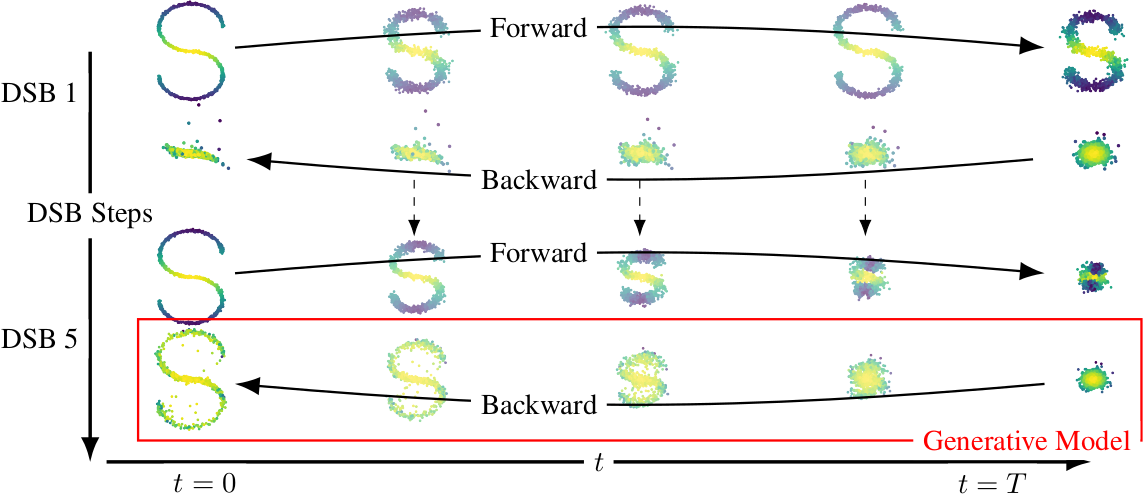
\includegraphics[width=\linewidth]{f/borto_shot1.png}
		\vspace{4em}

		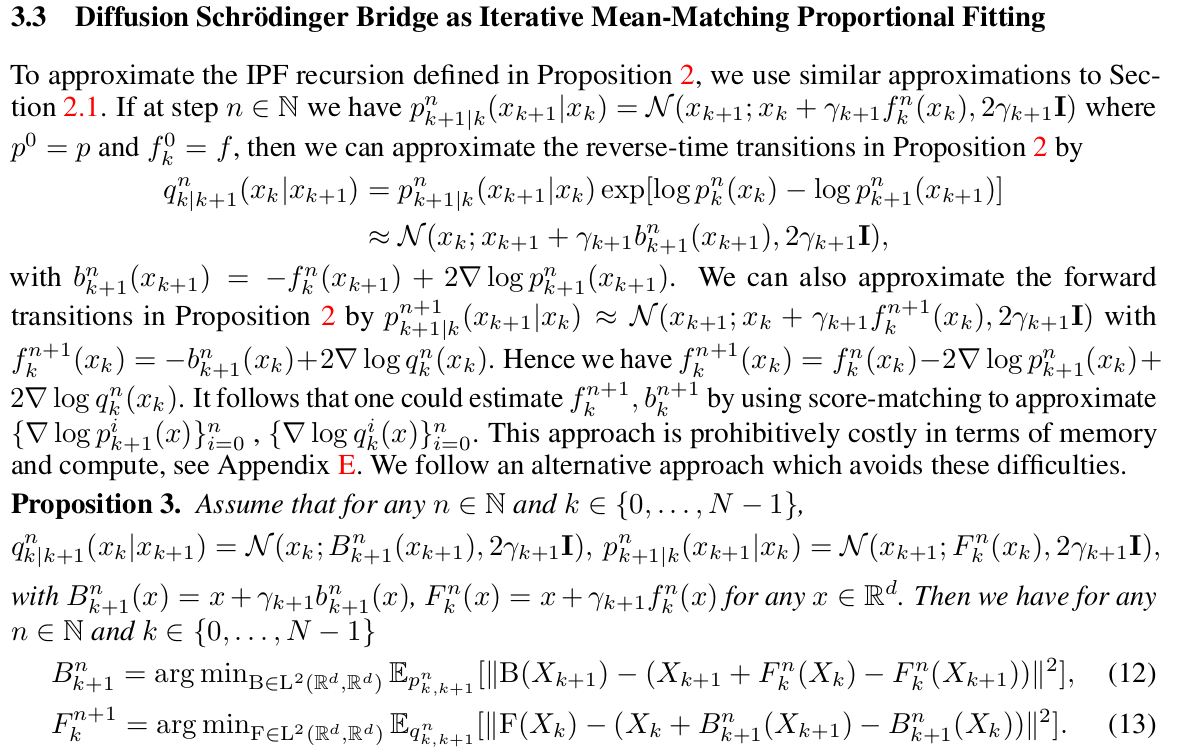
\includegraphics[width=\linewidth]{f/borto_shot2.png}
	\end{column}
	\pause
	\begin{column}{0.3\textwidth}\srcsize
		{\bf Zhe Zheng},
		{\color{gray} January 2024}\\
		{Denoiser and Its Application Beyond Denoising}
		\vspace{1em}

		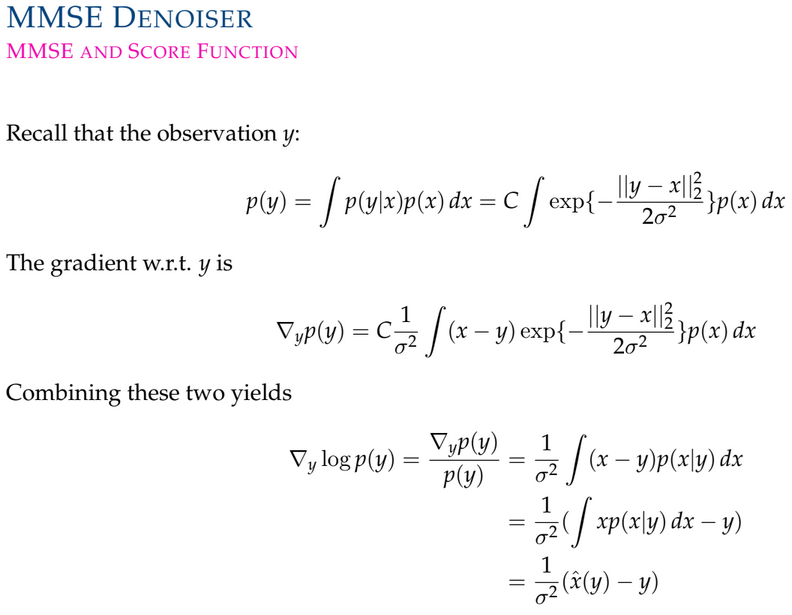
\includegraphics[width=\linewidth]{f/zhe_shot0.png}
		\vspace{1em}

		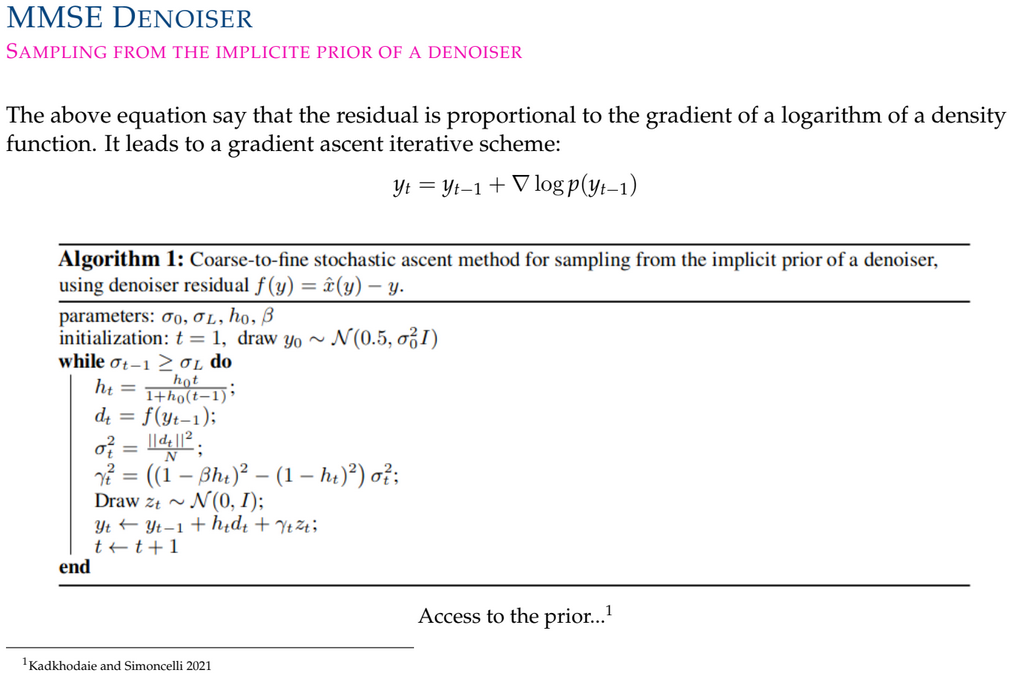
\includegraphics[width=\linewidth]{f/zhe_shot1.png}
		\vspace{1em}

		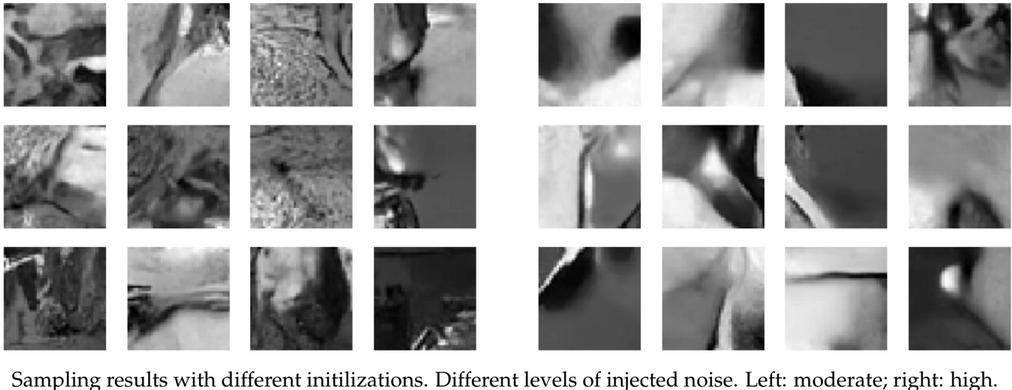
\includegraphics[width=\linewidth]{f/zhe_shot2.jpg}
	\end{column}
	\pause
	\begin{column}{0.3\textwidth}\srcsize
		{\bf Enric Meinhardt-Llopis},
		{\color{gray} February 2024}\\
		\vspace{4em}

		\pause
		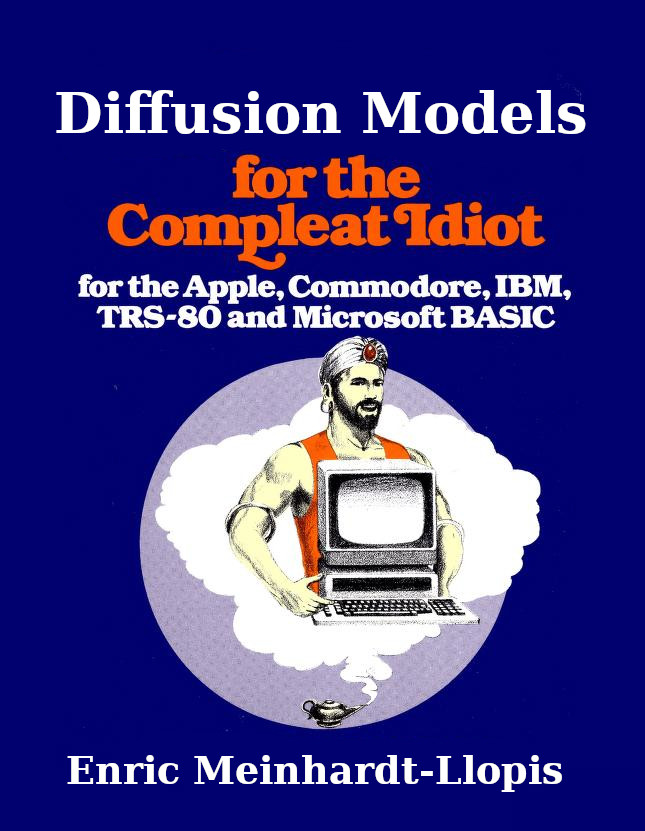
\includegraphics[width=\linewidth]{f/compleat.jpg}
	\end{column}
\end{columns}
\vfill
\end{frame}

\begin{frame}
CONTEXT: THE BASIC IDEA\\
=======================

\only<1>{
\vfill

\includegraphics[width=\linewidth]{f/gobrrr.png}
\vfill}\only<2-3>{
{\color{gray}Kadkhodaie-Simoncelli 2021}

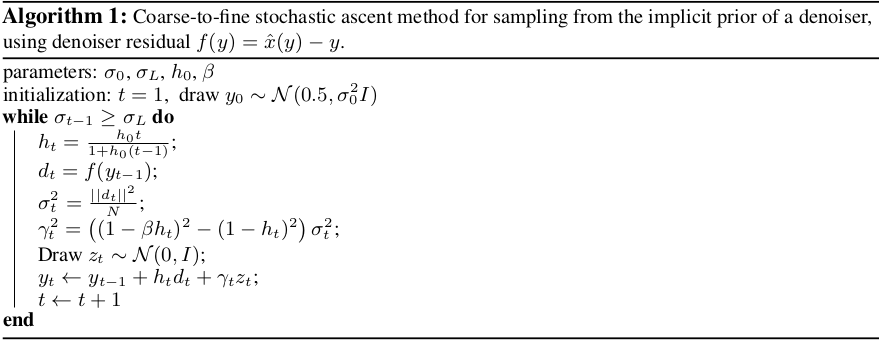
\includegraphics[width=0.9\linewidth]{ks.png}
}\only<3>{
	\vfill
\tiny
\begin{tabular}{lll}
	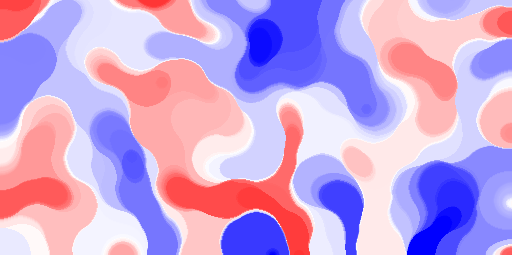
\includegraphics[height=0.18\textheight]{somiters3b.png} &
	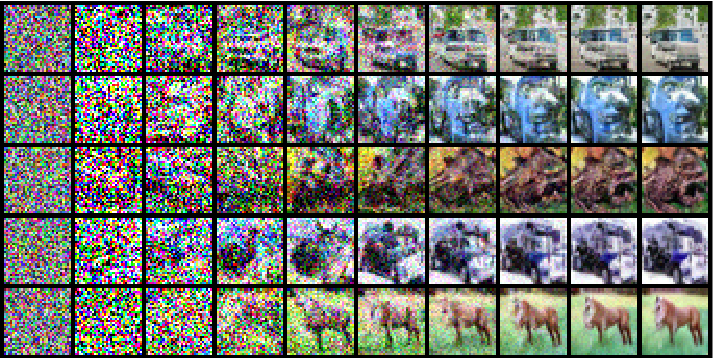
\includegraphics[height=0.18\textheight]{songermon1b.png} &
	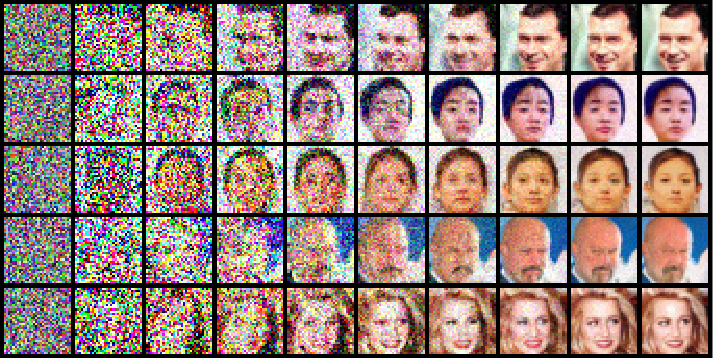
\includegraphics[height=0.18\textheight]{songermon1a.png} \\
	Denoiser = median &
	Denoiser = DCNN (generic) &
	Denoiser = DCNN (faces)
\end{tabular}
}
\end{frame}


\begin{frame}
OUTLINE\\
=======

\vfill

1. Implicit image priors by {\bf iterative denoising}\\
$\ \quad${\color{gray}($\approx$ 10min)}

2. Application to {\bf linear inverse problems}\\
$\ \quad${\color{gray}($\approx$ 5min)}

3. Colophon: implementation details\\
$\ \quad${\color{gray}($\approx$ 5min)}

\vfill

\end{frame}


% 1. iteration of denoisers
\begin{frame}%

\vfill
\begin{center}
\Huge
--1--\\Iteration of Denoisers
\end{center}
\vfill
\small
\centering
{And how each denoiser defines an implicit image prior}
\end{frame}


% 1.0 goal: understand the normalizations in K-S algorithm

% 1.1 what happens if we denoise an image iteratively?
% experiment using gaussian blur, without normalization
% experiment using gaussian blur, with normalization
% experiment using median filter, with normalization

% 1.2. review ks algorithm

% 1.3. algorithm written in terms of residual denoising
% alias X='plambda ``x x,V9 rot - 1 * x +'''
% alias X='plambda ``x,M9 x - 0.9 * x +'''
% plambda zero:128x128 randu|X|X|X|X|X|X|X|X|X|X|X|X|X|X|X|X|ntiply 10|d
% cat barbara.png|X|X|X|X|X|X|X|X|X|X|X|X|X|X|X|X|ntiply 10|d

% 1.4. link with heat equation

% 1.5. further links: moisan image iterative filtering, alvarez etal

% 1.6. recall main result of alvarez etal

% 1.7. interpretation of other steps in KS algorithm

% 1.8. experiments with various versions of parameters, classical denoisers

% 1.9. slightly fancier denoisers

% 1.10. the ks notebook





% 2. linear inverse problems
\begin{frame}%

\vfill
\begin{center}
\Huge
--2--\\Linear Inverse Problems
\end{center}
\vfill
\small
\centering
{And how can we solve them using a denoiser}
\end{frame}



% 2.0. linear inverse problems: definition
% 2.1. examples of linv problems: inpainting, spatial zoom-in, spectral zoom-in
% 2.2. see the modified algorithm
% 2.3. link with laplace inpainting
% 2.4. link with tv inpainting
% 2.5. examples with fancier denoisers


% 2. linear inverse problems
\begin{frame}%

\vfill
\begin{center}
\Huge
--3--\\Colophon
\end{center}
\vfill
\small
\centering
{implementation details}
\end{frame}


% 3.0. colophon: implementation details
% 3.1. show the ks source code (core algorithm)
% 3.2. show the ks source code (main function, with denoiser selection)
% 3.3. pip install ipol
% 3.4. local ipol run
% 3.5. idl and their shenanigans

% ending:
% k-s photos and links to presentations (IHES/simmons)
%
% Zahra Kadkhodaie
% Flatiron-Wide Machine Learning
% Flatiron Institute, June 2023
% https://www.youtube.com/watch?v=24IukBNPJLw
%
% Eero Simoncelli
% Photographic Image Priors in the Era of Machine Learning
% IHES, April 2023 (in honor of Mallat's birthday)
% https://www.youtube.com/watch?v=OiZFsn0_rjk






\end{document}

%\begin{frame}
%IMPLICIT IMAGE MODELS OF CLASSICAL DENOISERS\hfill{\footnotesize{\color{gray}mnhrdt}}\\
%============================================
%
%\small
%Any denoiser contains an ``implicit image prior''.\\
%How can we can extract images from it?
%
%{\color{gray}Kadkhodaie-Simoncelli 2021}\\
%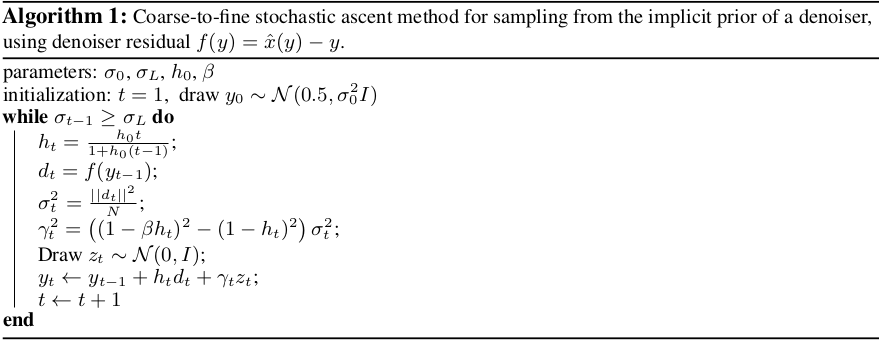
\includegraphics[width=0.7\linewidth]{ks.png}
%
%%\vfill
%{\bf Demo: } Bring your own denoiser for this algorithm
%
%%\vfill
%\tiny
%\begin{tabular}{lll}
%	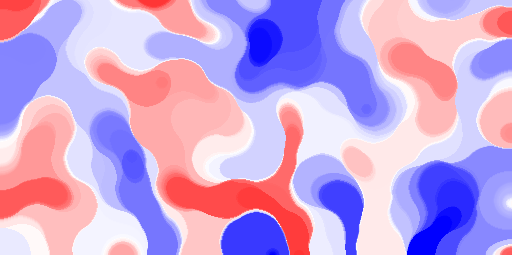
\includegraphics[height=0.18\textheight]{somiters3b.png} &
%	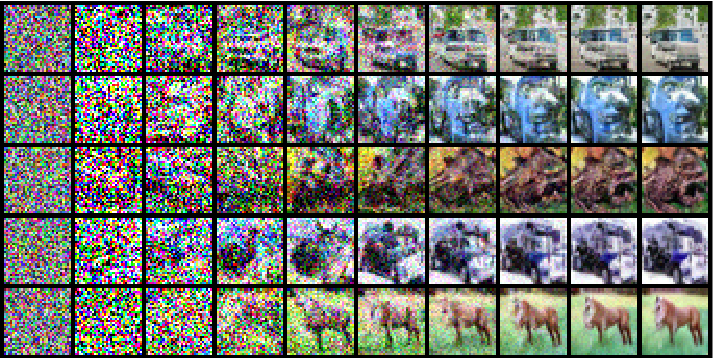
\includegraphics[height=0.18\textheight]{songermon1b.png} &
%	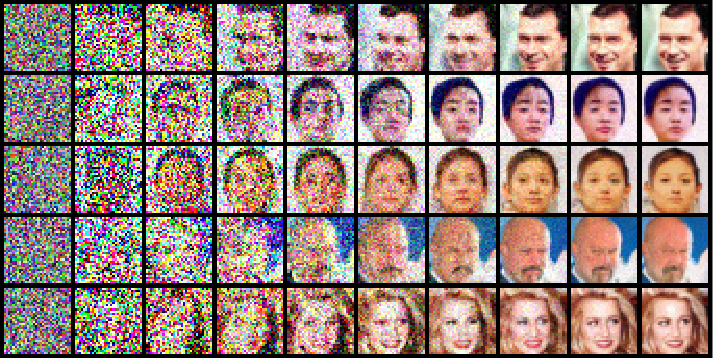
\includegraphics[height=0.18\textheight]{songermon1a.png} \\
%	Denoiser = median &
%	Denoiser = DCNN (generic) &
%	Denoiser = DCNN (faces)
%\end{tabular}
%
%\end{frame}
%
%\begin{frame}
%IMPLICIT IMAGE MODELS OF CLASSICAL DENOISERS
%============================================
%
%%Computed with current code:
%%Particular cases of Kadkhodaie-Simoncelli dynamics:
%
%\tiny
%\begin{tabular}{lll}
%	
\includegraphics[width=0.31\textwidth]{out_perlin.png} &
%	
\includegraphics[width=0.31\textwidth]{out_mcm.png} &
%	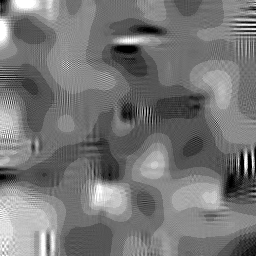
\includegraphics[width=0.31\textwidth]{out_dct.png} \\
%	gausssian blur (perlin noise) &
%	median filter (mcm) &
%	dct denoising \\
%	&&\\
%	
\includegraphics[width=0.31\textwidth]{out_nlm0.png} &
%	
\includegraphics[width=0.31\textwidth]{out_nlbayes.png} &
%	
\includegraphics[width=0.31\textwidth]{out_ffdnet.png} \\
%	non-local means (nl diffusion) &
%	non-local bayes &
%	ffdnet \\
%\end{tabular}
%
%\end{frame}
%
%\begin{frame}
%SUBPRODUCT: PYTHON INTERFACE TO IPOL ALGORITHMS
%===============================================
%
%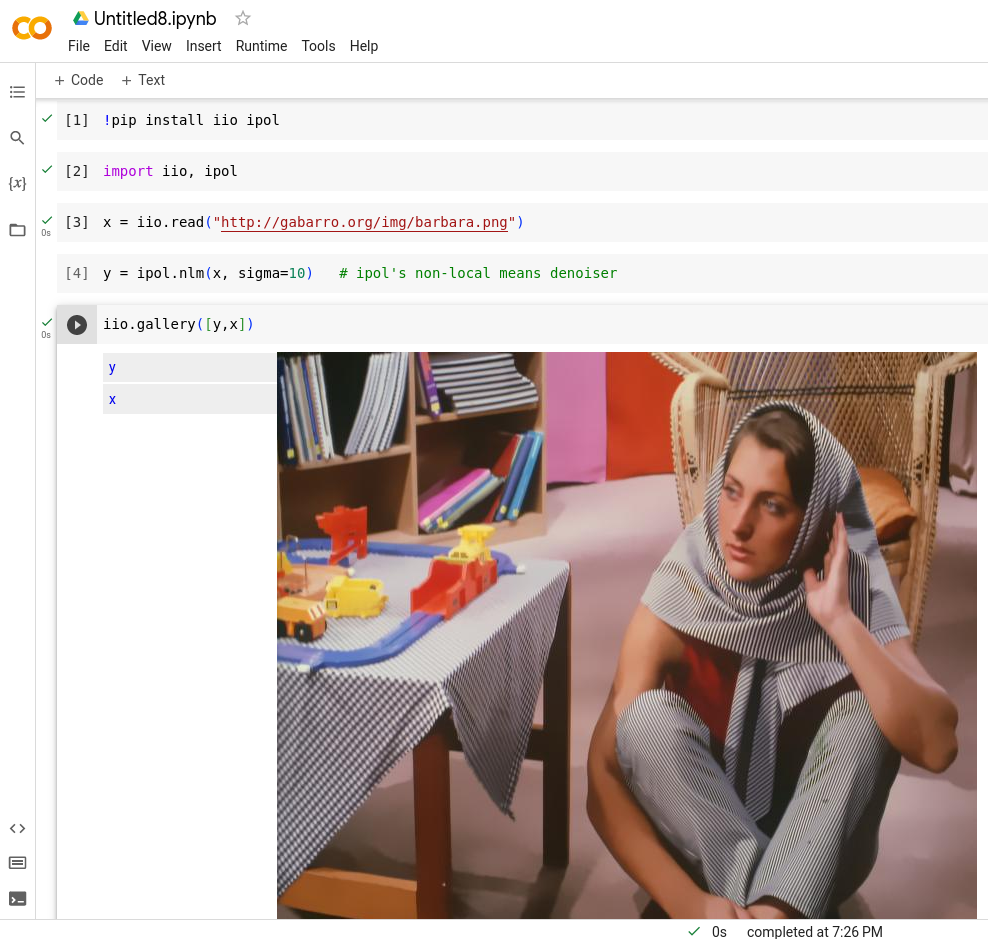
\includegraphics[height=0.9\textheight]{clipolcollab.png}
%\end{frame}
%
%
%\end{document}


% vim:sw=2 ts=2 spell spelllang=fr:
